\subsubsection{Rancangan Detail Komunikasi Antarnode}
\label{subsubsection:detail-komponen-internode-interface}

Komponen komunikasi antarnode bertanggung jawab untuk mengelola komunikasi antar node dalam sistem. Komponen ini berperan sebagai antarmuka yang digunakan komponen konsensus untuk berkomunikasi dengan node lain. Antarmuka akan berjalan menggunakan protokol TCP dengan abstraksi aplikasi dibuat secara manual. Hal ini dilakukan untuk meningkatkan kinerja dari sistem. Rancangan antarmuka komunikasi antarnode dapat dilihat pada Gambar \ref{fig:internode-interface-component}.

\begin{figure}[ht]
	\centering
	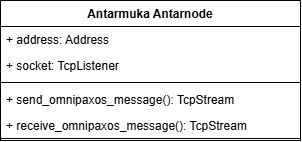
\includegraphics[width=0.45\textwidth]{resources/chapter-3/internode-interface-component.png}
	\caption{Komponen Antarmuka Komunikasi Antarnode}
	\label{fig:internode-interface-component}
\end{figure}

Antarmuka tersebut hanya menyediakan fungsi untuk mengirim dan menerima pesan. Abstraksi aplikasi yang perlu dilakukan adalah melakukan \textit{encode} pesan ke bentuk yang dapat dikenali oleh sistem dan \textit{multiplexing} agar pesan dari banyak sumber dapat diproses sesuai kebutuhan tanpa konflik dengan pesan lainnya mengingat pesan disimpan pada \textit{socket} yang sama menggunakan mekanisme \textit{queue}.